\documentclass[../main.tex]{subfiles}

\graphicspath{{\subfix{../imgs/}}}

\begin{document}

\section{Task 3.3}

Create two modules that realize a producer and a consumer thread. The modules should be connected together using a \textbf{sc\_fifo} channel. Use the structure of a TCP package to simulate the data transmitted over the transmission (fifo) channel. The producer transmits a new TCP package with a random interval between 2-10 ms. The consumer thread must print the simulation time and sequence number each time a new TCP package is received. Use the TCP Header structure as described below with a total package size of 512 bytes. Inspiration can be found in the \textbf{FifoFilter} (Fork.h, when adding two consumers) example project.


\begin{figure}[h]
    \centering
    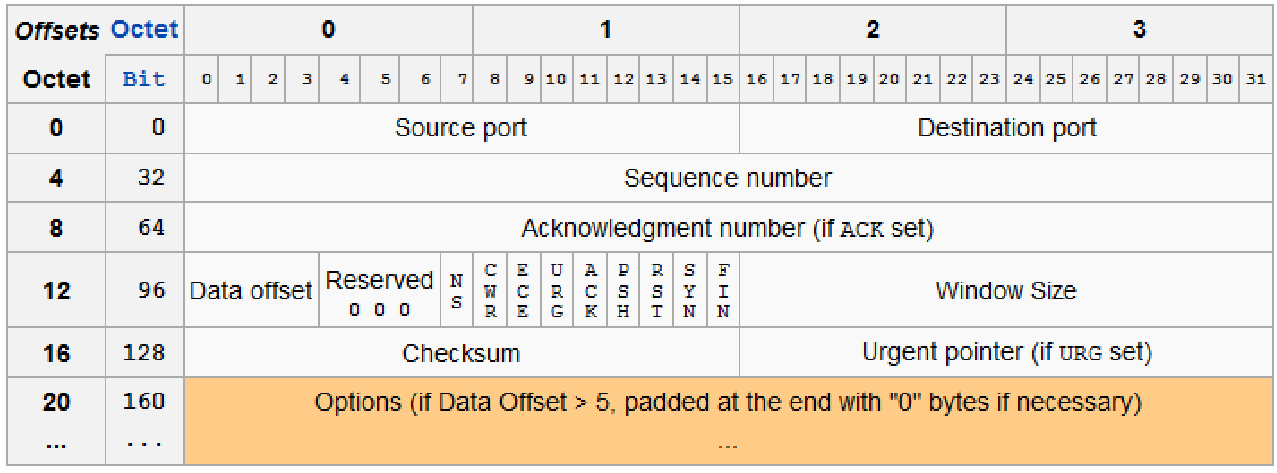
\includegraphics[width=0.9\textwidth]{task_3_3.png}
    \caption{TCP header structure.}
    \label{fig:tcp}
\end{figure}

Extend your model to have two fifo channels and consumers receiving TCP packes on port 1 and 2. The producer must be rewritten to connect to more ports.

\subsection*{Solution}

Let us start by describing the producer module \textbf{TCP\_Producer}. A simple class is defined with a thread \texttt{mainThread}, and a method, \texttt{transmit}, for transmitting TCP packets to all connected consumers.

\begin{myminted}{/inc/TCP\_Producer.hpp}
class TCP_Producer : public sc_module {
    public:
        sc_port<sc_fifo_out_if<TCPHeader*>, 0> out;
        sc_event event_transmit;
        TCP_Producer(sc_module_name name);
        ~TCP_Producer();
    
    private:
        std::string moduleName;
        void mainThread();
        void transmit();
    };
\end{myminted}

\texttt{mainThread} is simply waiting a random amount of time (between 2 and 10 ms) before notifying the \texttt{transmit} method by \texttt{event\_transmit}.

\newpage

\begin{myminted}{/src/TCP\_Producer.cpp - mainThread()}
void TCP_Producer::mainThread() {
    uint8_t wait_ms = 0;
    while (true) {
        wait(wait_ms, SC_MS); 
        event_transmit.notify();
        wait_ms = rand() % 9 + 2;
    }
}
\end{myminted}

\begin{myminted}{/src/TCP\_Producer.cpp - transmit()}
void TCP_Producer::transmit() {
    TCPHeader* packet = new TCPHeader();
    packet->SourcePort         = 0;
    packet->DestinationPort    = 0;
    packet->SequenceNumber     = 0;    
    packet->Acknowledge        = 0;
    packet->StatusBits         = 0;
    packet->WindowSize         = 0;
    packet->Checksum           = 0;
    packet->UrgentPointer      = 0;
    memset(packet->Data, 0, DATA_SIZE);

    for (int i = 0; i < out.size(); i++) {
        TCPHeader* packet_copy = new TCPHeader(*packet);
        packet_copy->DestinationPort = i;
        out[i]->write(packet_copy);
        std::cout << moduleName << ": transmitting packet to port " << packet_copy->DestinationPort
                  << " - time: " << sc_time_stamp() << '\n';
    }
    delete packet;
}
\end{myminted}



\end{document}

